The algorithm that is implemented in the scope of the thesis is in principle the one from \textcite{Derrac2015}, but includes some improvements from \textcite{Ager2018} and \textcite{Alshaikh2020} - both of which directly builing on the work of the former. As all of these publications share Prof. Steven Schockaert as last author, it seems plausible that a) the latter ones are legit improvements upon the first, b) at least to a certain degree they can share code and data, c) this field of work is constrained to a small community, without any alternative implementations or substantial improvements from outside of it.
% sollte ja schon vorher erwähnt haben dass das thema leider nicht über diese small community hinaus geht
% and includes my own improvements und anpassungen für den speziellen datensatz
% und ist so modular wie möglich

\subsection{Core Idea}

% The core idea of the algorithm is to unsupervisedly find a a set of features which can be modelled as directions for a vector-space representation of the respetive entities.
The main goal of the algorithm is to unsupervisedly use the considered text-corpora associated with the respective entities from a certain domain % descriptions, reviews, ...
to embed the entities in to a vector-space where the axes correspond to human concepts, % "concepts" meaning attributes and what-was-the-other-again, according to CS lingo corresponding to nouns and adjectives, TODO: see above where I described that already.
allowing a \textit{feature-based} representation of them - a high-dimensional vector that numerically encodes the degree % protypicality
to which the entity corresponds to a number of appropriate dimensions. % Das haupt-ziel der algorithmen ist es, am ende die entities "feature-based" darstellen zu können, also als high-dim-vector mit floats per human-interpretable dimension. 
% Alshaikh2020 hat dafür wegen den subfeatures noch kleine specials
\newline

The general idea to achieve that is as follows: First, the entities %TODO: at this point already defined that entities = texts = descriptions/concatenatedreviews/... 
are embedded as fixed-dimensional vectors. This already softens the definition of a conceptual space, as the considered entities are modelled as vectors instead of regions. % entities were supposed to be regions, however here we assume vectors because it's computationally a lot easier (TODO: are the reasons mentioned elsewhere? also the distiction between types and tokens?)
To allow for the types of reasoning mentioned in Section \ref{sec:cs_reasoning}, %TODO: section where the entire mapping from logic-reasoning to CS-reasoning is explained, mostly from DESC15 and Gärdenfors himself
it is embedded into metric spaces where the concepts of direction and distance are well-defined. \gencite{Derrac2015} original algorithm uses MDS (see \ref{MDS}) for this matter, which enforces equal distances  %TODO: link the distance-matrix-notepad FROM MY REPO in nbviewer+binder
(however as shown by \textcite{Mikolov:Regularities}, such things are also possible with neural word-embedding techniques such as word2vec \cite{Mikolov:Word2Vec}) %TODO: word2vec cite
. Additionally, words from the text are extracted as candidates for the names of the semantic dimensions. The core assumption is then, that \q{words describing semantically meaningful features can be identified by learning for each candidate word $w$ a linear classifier which separates the embeddings of entities that have $w$ in their description from the others} \cite[3574]{Alshaikh2020}. The better the performance of that classifier according to a chosen metric, the more evidence there is that $w$ describes a semnatically meaningful feature. 
% * from Alshaikh2020: "Their core assumption is that words describing semantically meaningful features can be identified by learning for each candi- date word w a linear classifier which separates the embeddings of entities that have w in their description from the others. The performance of the classifier for w then tells us to what extent w describes a semantically meaningful feature"
% TODO: make the direct quote shorter, such things should only be done "to support an argument", which I don't here.
In a final step, the candidate-words are clustered according to their similarity to find a fixed set of dimensions. A representative term for the directions is selected, and the entities are re-embedded into a new space comprised of these dimensions, where the individual vector-components correspond to the ranking of an entity with respect to these dimensions.
% * from Alshaikh2020: "The learned vectors will be referred to as feature directions to emphasize the fact that only the ordering induced by the dot product d_i · e matters"
\newline

\todoparagraph{Important features:} %TODO:
\begin{itemize}
	\item Unsupervised, data-driven (in contrast to \textcite{VISR12})
	\item Modular (subcomponents may be exchanged)
	\item Optimize for "looking good to humans", so no straight-forward metrics or obvious way to evaluate
\end{itemize}


Many of the just mentioned components don't refer to a specific algorithms, and the existing implementations \mainalgos differ in many of these implementations. The rest of this sections goes into further detail for each of these components, and an overview of the components supported in the respective implementations is given in \tref{tab:compared_algos}. Further, configuration files to enable exactly the respective components of the respective papers for the codebase of this thesis are listed in \aref{ap:yamls_for_origalgos}.


% #########################################################################################################################################################################################################################################################################################################################################################################################################################################################################################################################################################################################################################################################################################################################################################################################################################################################

\subsection{Steps of the algorithm}

% TODO: THIS from \cite{Turney2010} is a very fucking good explanation!!!

% After the text has been tokenized and (optionally) normalized and annotated, the first step is to generate a matrix of frequencies. Second, we may want to adjust the weights of the elements in the matrix, because common words will have high frequencies, yet they are less informative than rare words. Third, we may want to smooth the matrix, to reduce the amount of random noise and to fill in some of the zero elements in a sparse matrix. Fourth, there are many different ways to measure the similarity of two vectors. Lowe (2001) gives a good summary of mathematical processing for word–context VSMs.
% He decomposes VSM construction into a similar four-step process: calculate the frequencies, transform the raw frequency counts, smooth the space (dimensionality reduction), then calculate the similarities.

The considered algorithm first embeds the collection of texts into a vector space, to afterwards extract important features from this space using linear classifiers. The second step is an original idea of \cite{Derrac2015}, however creating vector space embeddings from texts is a very popular technique, used for many tasks in computational linguistics \cite{Mikolov:Regularities,Mikolov2013a,Guo,Lowe,Turney2010}. %TODO: irgendwo bin ich ja noch auf word2vec und den ganzen bums eingegangen blabla, nochmal schreiben dass es hier um classical AI geht und ebennicht die sahcen wie word2vec und glove
%TODO: glove und fasttext cite?!

 \textcite{Lowe} conceived a general framework to construct vector spaces from texts, splitting the process into the steps of first counting the token frequencies, then transforming the raw counts into more useful \gls{quant} measures (see \ref{sec:word_count_techniques}) %adjust the weights of the elements in the matrix, because common words will have high frequencies yet are less informative than rare words.
 %TODO: talk about a fucking DOC-TERM-MATRIX, A MATRIX OF FREQUENCIES!!!
  and smoothing the space using dimensionality reduction, before calculating the similarities on the resulting embedding. While the considered algorithm requires more steps before calculating the similarities to allow for domain-specific and more complex forms of reasoning, it also adheres to this structure, as will be shown in section~\nameparanref{sec:generate_vectorspaces}.

%TODO:
% * reference yamls again
% * Im Text link zu binder bei results section der auf die notebooks/analyze_results/analyze_pipeline_results.ipynb referenziert, und für die tables auch!
% * Schreiben dass ich einige Claims oder nonclaims von denen prüfe, bspw nutzen sie immer PPMI ohne je tf-idf zu testen
% * Wie lange der ganze Kram dauert - MDS hat quadratic complexity etc
% * Das mit dem Koordinatensystem drehen passiert gar nicht so wie ich dachte dass es passiert...?!
% * Tabelle
% 	* Einduetig rausschreiben welche der 3 paper [DESC15] [AGKS18] [RaZb20] welche parameter-werte verlangen und !!welche optimal waren!! angucken welche Kombi die Beste Performance hatte und die entsprechend markieren (und im yaml haben!)!


% 	* POSSIBLE EXTRA-STEPS FOR ALGORITHM
% 		* BOOTSTRAP MORE CANDIDATES (AFTER EXTRACT CANDIDATES)
% 			* [VISR12]: LSI
% 				* Options:
% 					* What to take for the term-document-matrix
% 						* [VISR12]: 
% 							* tag-applied
% 							* tag-count
% 							* tag-share (the number of times tag t has been applied to item i, divided by the number of times any tag has been applied to item i)
% 						* relative-tag-count (tag-count / text-len) or tag-count / distinct-words-in-text
% 						* See also: https://en.wikipedia.org/wiki/Latent_semantic_analysis#Term-document_matrix
% 				* Parameters:
% 					#dims for the rank reduction (see https://en.wikipedia.org/wiki/Latent_semantic_analysis#Rank-reduced_singular_value_decomposition)

% * Schritte des Algorithmus bewerten:
% 	* "that the better Ht separates entities to which t applies from the others in S,the better \vec{v_t} models the term t." --> wie sinnvoll ist diese measure wenn das verhältnis literally 14.900 zu 100 ist, dann haben halt 99.33% der Daten einen rank von 0 ?!
% 	* DESC15 write they select Kappa "due to its tolerance to class imbalance." -> Does that mean I have to set the weight?! Außerdem weiß ich ja superviel ebennicht, like which weighting they use! I don't like
% 	* Der letzte Schritt mit dem Clustern der good-kappa-ones ist wirklich very basic und hat very much room for improvement



%TODO: maybe describe shortly what the improvements from  Ager2018 Alshaikh2020 were? 

% * Regarding DESC15 vs AGKS18 vs Alshaikh2020:
% 	* didn't somebody say that cohen's kappa sucks!?!
% 	* Alshaikh2020: 
% 		* use affinity propagation "for getting rid of the clusters of informative words", similar to how they did it in their 2019 paper
% 			-> affinity propagation has a so-called preference parameter, den als config lassen - usual, this parameter is chosen relative to the median µ of the affinity scores. For the methods Sub and Or- tho, we considered values from {0.7µ, 0.9µ, µ, 1.1µ, 1.3µ}
% 		* do kappa ON BINARY!!!
% 		* say that for them, the binary "does the word occur in the description" is the only sensible signal, no ppmi or anything! (page 2, footnote 1 of RaZb20)
% 		* "When representing a particular entity in a conceptual space, we need to specify which domains it belongs to, and for each of these domains we need to provide a corresponding vector." 
% 		* then they show their example of something that is not seperable with a hyperplane unless we specify subdomains, maybe just steal their plot that explains their one contribution to 99%
% 	* DESC15: 
% 		* "Here we use the assumption that the better Ht separates entities to which t applies from the others in S,the better \vec{v_t} models the term t." --> allein von der aussage muss man das mit den induzierten rankings echt nicht machen, sondern halt nur auf classification quality (-> metrics like accuracy) gucken, bzw kappa anhand der binären klasse berechnen --> the ranking induced by count, or the baremetal count?
% * The "Disentangled" from their title means "feature-based"


The core idea of the algorithm is to (unsupervised, data-driven) find a a set of features which can be modelled as directions for a vector-space representation of the respetive entities. For that, the steps are:

\begin{enumerate}
	\item preprocess the descriptions using default techniques and create a bag-of-words representation for the texts
	\item extract candidate features from these texts (easist variant is to just consider each sufficiently frequent word as candidate)
	\item create a fixed-dimensional embedding for the texts (optimally a metric space, optimally based on their dissimilarity)
	\item for each candidate term, train a linear classifier to seperate the vector representations of the entities that contain the term vs those that don't. If some metric for this classifier is sufficiently high, assume that the candidate term captures a salient feature - it's direction is then characterized by the normal vector for that hyperplane (for an intuition see \ref{fig:3d_hyperplane_ortho})
	\item Cluster the candidates and re-calculate the directions
	\item (optionally) Post-process the clusters 
	\item Calculate the direction of the cluster from the directions of it's contents to create a new space to embed the entities into
\end{enumerate}

% MENTION IN STEPS
%   3) fixed-dimensional embedding: 
%		* RaZb20 tried Doc2Vec instead of MDS and it performed worse!
%   5) if metric, assume salient:
%  		* [AGKS18] haben den candidate-filter-teil konfigurierbar (und sagen bei denen ist accuracy even better than kappa)

\fref{fig:dependency_graph} shows an automatically exported dependency_graph-graph, displaying the individual steps of the algorithm as done in the codebase of this thesis, also showing where selected important parameters are first used. As explained in section \ref{sec:architecture}, the modularity of the provided architecture allows individual components to be exchanged as needed.
\todoparagraph{I should also refer to} \tref{tab:compared_algos} here!


\begin{figure}[htp]
	\begin{center}
	  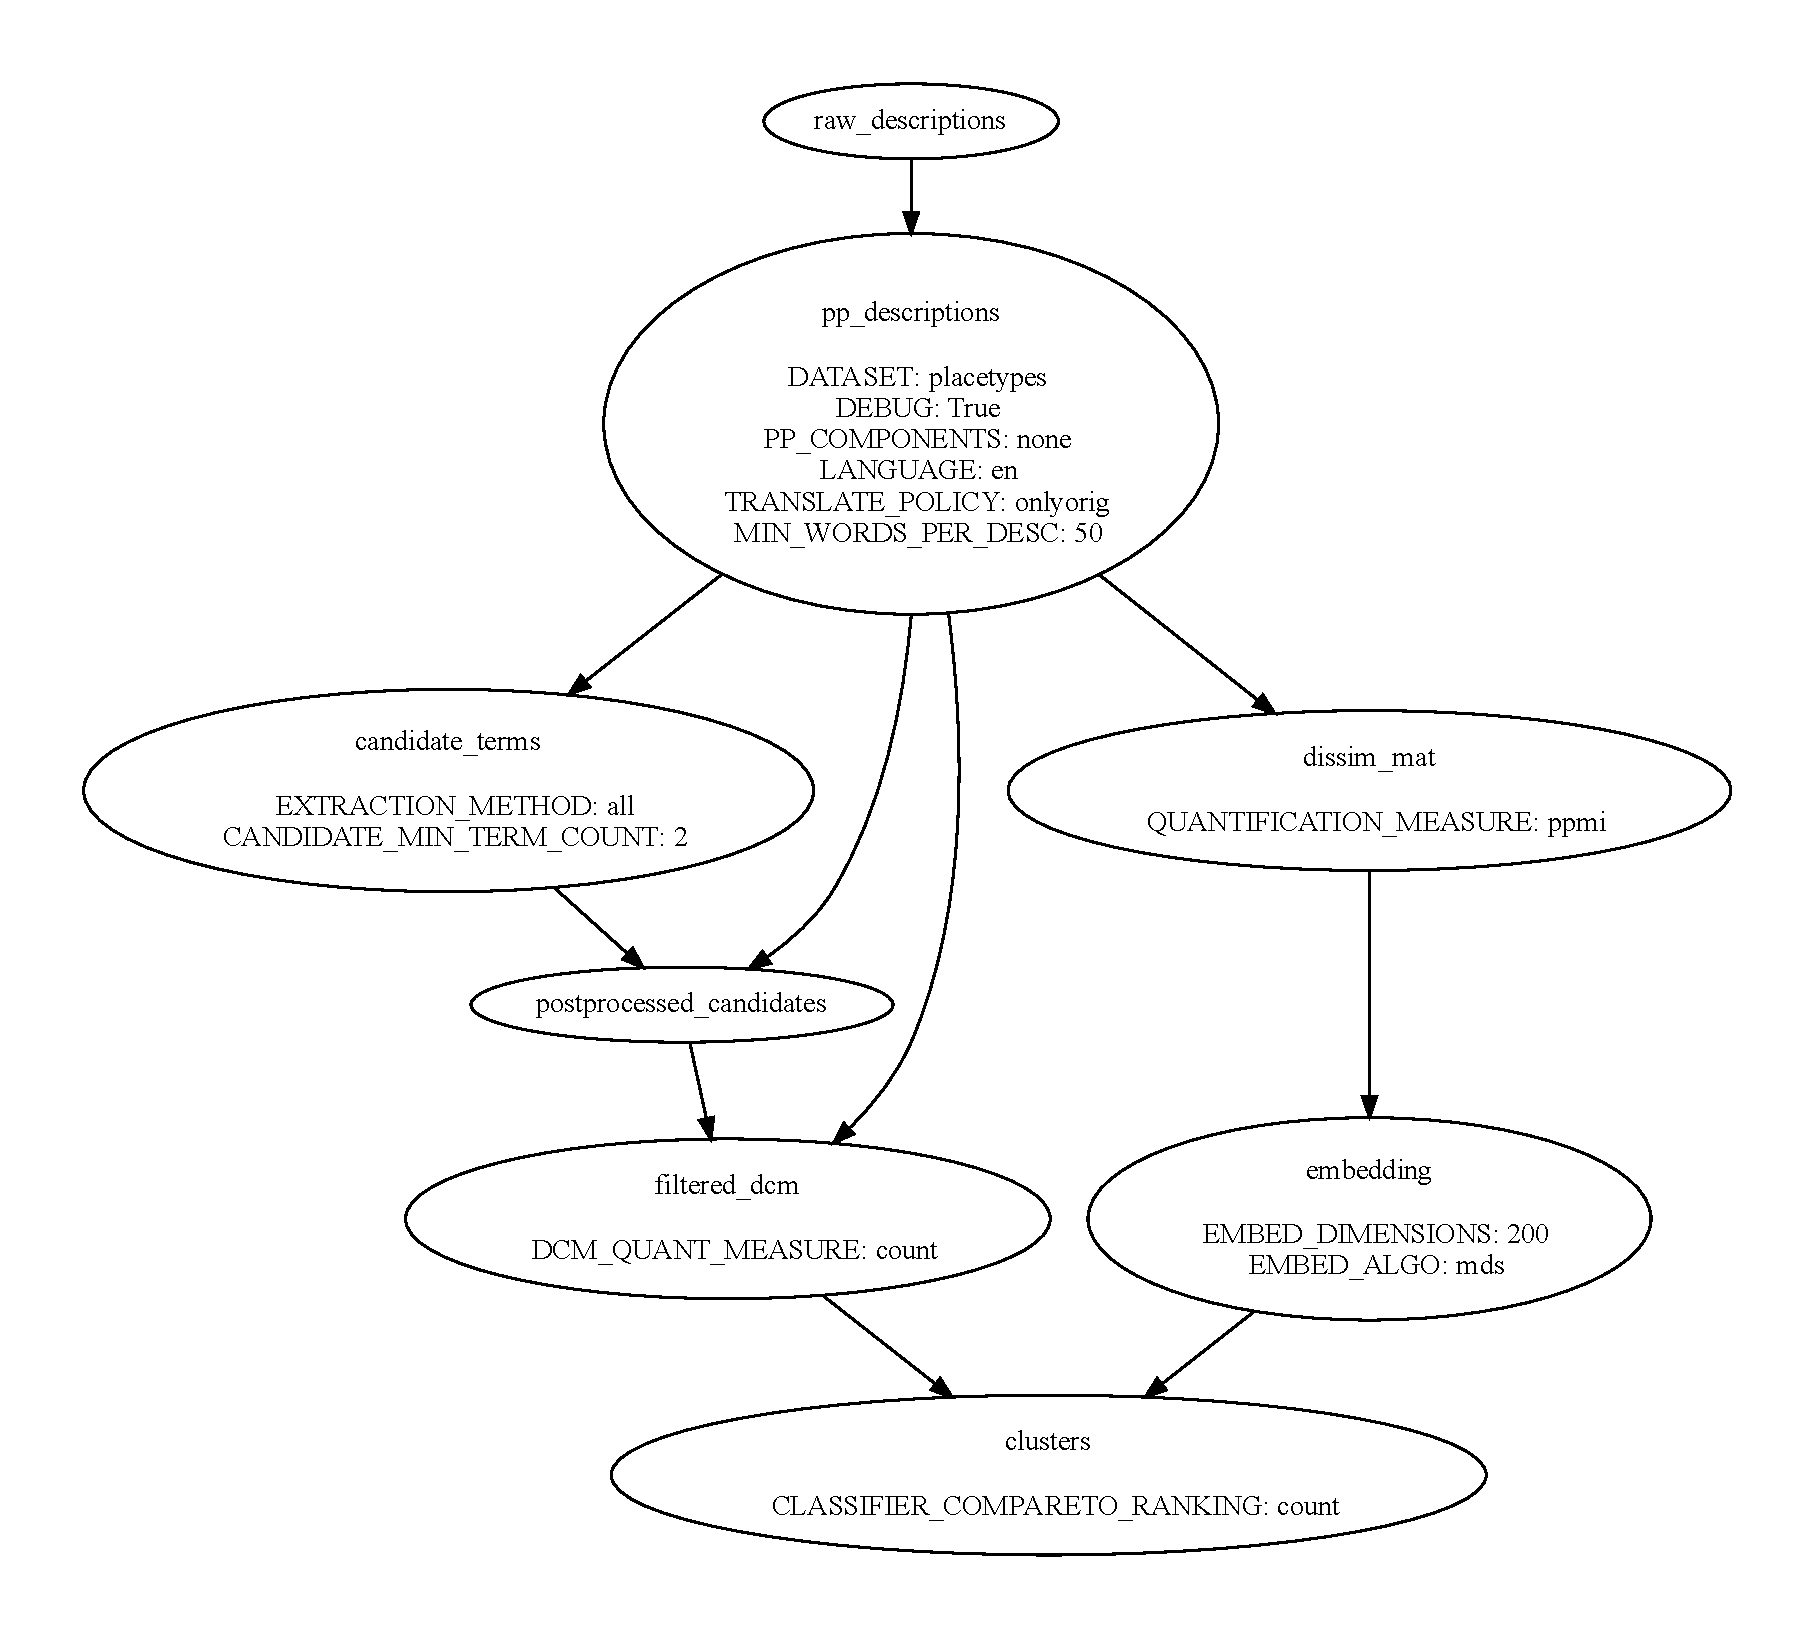
\includegraphics[width=0.9\textwidth]{dependency_graph_2022-02-14_11-36-45}
	  \caption[Dependency-Graph of the Algorithm]{(automatically generated) dependency-graph, displaying the individual steps of the algorithm as well as their dependencies and where selected important parameters are first used.}
	  \label{fig:dependency_graph}
	\end{center}
\end{figure}





\begin{landscape}
	\begin{table}[]
		%Preprocessing siehe other table
		\resizebox{\textwidth}{!}{%
			\begin{tabular}{lllll} % statt textcite mit \fancyquotecite https://tex.stackexchange.com/a/468286/108199
			& \textbf{\textcite{Derrac2015}} & \textbf{\textcite{Ager2018}} & \textbf{\textcite{Alshaikh2020}} & \textbf{This codebase} \\

			\textbf{Step 1: Generate Vector Spaces (Embeddings) from Descriptions} 
			& 
			\specialcell[l]{MDS trained with the angular differences $\frac{2}{\pi}* arccos\left(\frac{\vec{v}_{e_i}*\vec{v}_{e_j}}{\norm{\vec{v}_{e_i}}*\norm{\vec{v}_{e_j}}}\right)$ \\
				between the PPMI weighted BoW Vectors (all terms) \\
				Spaces of dim 20, 50, 100 and 200 \\
				Previous Experiments also considered SVD and Isomap}
			&
			\specialcell[l]{ \tabitem like \cite{Derrac2015} 
				\\ \tabitem PCA from PPMI weighted BoW vectors (no quadratic complexity) \\ \tabitem Doc2Vec\footnote{\label{foot:doc2vec} TODO: Explain and cite!} Document Embeddings \\ \tabitem thresholded\footnote{\label{foot:threshold}Only words that occur more than 2 times (15 for movies-dataset)}, averaged pre-trained GloVe word embeddings \\ \tabitem thresholded\footref{foot:threshold}, PPMI-weighted-averaged pre-trained GloVe word embeddings \\
				Number of dimensions one of (50, 100, 200)}
			&
			\specialcell[l]{ \textbf{movies and placetypes:} Re-used the 100D-embeddings of \textcite{Derrac2015} \\ \textbf{other datasets}: \\ \tabitem 100d Document Embeddings from angular differences and MDS\\  \tabitem 100d-Doc2Vec\footref{foot:doc2vec} }
			& 
			\specialcell[l]{ \tabitem MDS, \tabitem t-SNE or \tabitem Isomap with arbitrary number of dimensions \\ on a dissimilarity-matrix based on \tabitem BoW (raw counts), \tabitem BoW (binarized), \tabitem tf-idf-weighted BoW, \tabitem ppmi-weighted BoW, \tabitem tf-weighted BoW \\ distance measure \tabitem normalized angular distance \tabitem cosine distance \tabitem TODO: the other distance measures}
			\\ \midrule

			\specialcell[l]{ \textbf{Step 2: Generate Candidate Words} \\ \textbf{for Feature Directions} } 
			& 
			\specialcell[l]{ All sufficiently frequent\footnote{For the placetypes-dataset: all tags that co-occur with at least 50 place types} adjectives, nouns, adjective phrases and noun phrases \\
				(using POS-Tagger and Chunker from openNLP) } 
			&  
			\specialcell[l]{All sufficiently frequent words\footnote{For the thresholds, see table \ref{tab:all_datasets}} (use PPMI in a later step so possibly PPMI?!) \\ weighted Logitistic Regression Classifier for Vector Direction} 
			&
			\specialcell[l]{ 
				\textbf{Candidates:} movies and placetypes: see \textcite{Derrac2015}, other datasets: all occuring\footnote{see Datasets-Table} 1-grams \\
				\textbf{Classifier:} logistic regression classifier (similar performance to SVM but faster training)
			}
			&
			\specialcell[l]{ Keywords extracted using \\ KeyBERT (on \tabitem raw or on \tabitem preprocessed texts) \\ \tabitem all sufficiently frequent phrases \\ Those with a minimal score for \tabitem PPMI \tabitem tf-idf \tabitem tf}
			\\ \midrule


			\textbf{Step 3: Filter Candidate Feature Directions} 
			&                   
			\specialcell[l]{ linear SVM for all candidates (pos samples: $\forall e: c \in e$) with pos/neg-count-ratio as instance cost \\
				Only take candidates where the correlation according to Cohen's Kappa between the ranking induced by the SVM's hyperplane and count(t, e) is $\geq \lambda$ (0.5/0.1)\\
				also tried Spearman's and Kendall's correlation coeffcients }
			&
			\specialcell[l]{ Classifier-Performance as measured by \\ 
				\tabitem Cohen's Kappa (compared to the ranking induced by the PPMI) \\ \tabitem Accuracy (binary)\\ \tabitem Normalized Discounted Cumulative Gain (NDCG) (TODO: binary? ranking?) } 
			& 
			\specialcell[l]{
				Cohen's Kappa (threshold=0.3 in iteration 1 and 0.1 in iteration 2), only the top 5000 scoring features
			}
			& 
			\specialcell[l]{ 
				Various classifiers such as \tabitem linear SVM \tabitem squared-hinge-loss-SVC \\ %TODO: add SVC to acronyms. TODO: see Complexities of SVM implementations in python: https://stackoverflow.com/a/64274403/5122790 TODO: it's really easy to add the classifiers of \cite{Ager2018} & \cite{Alshaikh2020}, low-hanging fruit! 
				Compare classifier performance with \tabitem count \tabitem tf-idf \tabitem PPMI \tabitem \dots \\
				Comparison Functions: \tabitem Accuracy, Precision, Recall, F1 \tabitem Cohen's Kappa (rank2rank) \tabitem Cohen's Kappa (various other ways)
			}
			\\ \midrule


			\textbf{Step 4: Merge Feature Directions} 
			&   
			\specialcell[l]{ According to \cite{Alshaikh2020} "a variant of \textit{k}-means" \\ Cluster centers: Select Term with highest $\kappa$, then i=2*ndims times select the term from $T^{0.5}$ minimizing $max_{j<i}cos(\vec[m]{v_{t_j}},\vec[m]{v_t})$ \\ 
				Others: assign all terms from $T^{0.1}$ to the closest cluster and define $\vec[m]{v^*_i} = \frac{1}{|C_i|} \sum_{t\in C_i} \vec[m]{v_t}$ as cluster direction (average direction of cluster's elements)} 
			&
			\specialcell[l]{Input-ndims for clustering algorithm one of (500, 1000, 2000) \\
			Number of clusters one of (ndims, 2*ndims) \\
				Centroid of the cluster computed as $v_{C_j} = \frac{1}{|C_j|}\sum_{w_l \in C_j} v_l$, provided $\vec[m]{v_w}$ all normalized} 
			& 
			\specialcell[l]{  \textbullet\, \textbf{sub, ortho, primary}:   
				Affinity propagation instead of \textit{k}-means (no need to specify the ndims, helps with the issue that there are some non-informative clusters in \cite{Derrac2015}'s algorithm) \\ ~~ n-dims for this not directly configurable, only over preference parameter relative to median $\mu$, tried for (0.7$\mu$, 0.9$\mu$, $\mu$, 1.1$\mu$, 1.3$\mu$) \\  \textbullet\, \textbf{AHC}: Agglomerative Hierachical Clustering to cluster word directions with distance cut-offs  \\ \textbullet\, also tried Hierachical LDA \\ Cluster direction (AHC and Affinity Propagation): normal vector of the hyperplane of a linear classifier separating entities whose description contains at least one of the words from the cluster from the others  } %TODO find a short-term notation for "entities whose description contains at least one of the words from XYZ" ("for a Cluster C, we write pos_C and neg_C for the set of positively and negatively classified entities")
			&
			TODO: my stuff
			\\  \midrule

			\textbf{Step 5: Post-Processing} 
			&                   
			None 
			&                 
			TODO describe fine-tuning! 
			& 
			\specialcell[l]{
				Perform steps 1-4 a second time (only for positively classified entities), such that there are primary features (domains) and sub-features \\ representation kept flat (values for the sub-features is same dot-product as for domains) \\ \textbullet\, \textbf{sub}: sub-features extracted equal to first-order-features \\ \textbullet\, \textbf{ortho}: sub-feature directions orthogonal to corresponding primary feature direction (enforce complementary information) \\ ~~ by computing orthogonal decomposition of feature w.r.t. its domain (pg. 4, equation 1) \\ \textbullet\, also tried to combine mother-domain with sub-feature, but that performed poorly \\ \textbullet\, \textbf{primary}: model with only primary features}
			&
			TODO: my stuff
			\end{tabular}
		}
		\caption{Compared algorithms from \cite{Derrac2015} \cite{Ager2018} \cite{Alshaikh2020}}
		\label{tab:compared_algos}
	\end{table}
\end{landscape}

% Alshaikh2020 say: "It may seem counter-intuitive to use binary classifiers to learn representations of ordinal features. However, the occurrence or non- occurrence of a word in the description is binary, and this is the most important available signal. We experimented with statistics such as pointwise mutual information, which did not lead to better results." -> does that mean DCM_QUANT_MEASURE or QUANTIFICATION_MEASURE or both? and also does that mean they use binary or count as this measure?

% Alshaikh2020 use: sub, ortho, primary, random (coordinates uniformly random), 


Before looking at the steps in turn, it should be noted that even the preprocessing does not work on completely raw data, but on curated and processed corpora. This processing is however not considered part of the algorithm, as it is very specific to the respective datasets and manual dataset exploration, tweaking settings such that they are best for the respective corpora\footnote{Because of this, it was done in sepearate Jupyter Notebooks, such as \url{https://github.com/cstenkamp/derive_conceptualspaces/blob/main/notebooks/create_datasets/Preprocess_Siddata2022.ipynb} }. %TODO: instead link to nbviewer/binder!!


\subsubsection{Preprocessing}

\label{sec:algo_preproc}

The first step of basically all NLP algorithms must be to pre-process the text corpus. The preprocessing itself consists of multiple independent components chained after each other. Which components are necessary also depends on the processed dataset - as for example the \emph{placetypes-dataset} consists of a collection of tags instead of full sentences, tokenizing sentences or removing \glspl{stopword} becomes irrelevant. Other datasets may require additional cleaning or are already available in preprocessed form.
% * some parts of this depend on the dataset 
%     * Some may just require additional cleaning (remove HTML-Tags and such things)
%     * Some are already mostly preprocessed (placetypes is already a bag-of-words so there's not much to do there, and we skip almost all preprocessing-steps)
%     * In course-descriptions, I want some parts of the pre-preprocessing be part of the pipeline, like how we merge descriptions of different iterations of the same course that overlap to a high degree (sentwise-merge vs relative-term-frequencies)

As the main considered dataset of university-courses is highly multilingual (see \autoref{fig:courses_language_distribution}), one of the first questions that needs to be addressed is how entities of different langauges are handled. The algorithm consists of classical language processing algorithms such as comparing \gls{bow} representation of the entities, which means that the same text in two different languages may result in maximally different representations\footnote{\todoparagraph{another reason that makes checking out word2vec worth it!}}. Because of this, before any other processing, the languages of the entities is checked, such that entities of languages other than the demanded may be either translated, left out or used anyway\footnote{For details about the translation-step, it is referred to Appendix \ref{ap:translating}. It should be noted that professional automatic translation is costly and thus not all texts are available in all languages.}.

\FloatBarrier

The following components are developed for the preprocessing, every one of which can be individually enabled or disabled:
\begin{itemize}
	\item Prepend title and/or subtitle to the entities' associated text \itemtext{useful for the SIDDATA-Dataset, as the titles are often quite long and more descriptive than their descriptions}
	\item Remove HTML-Tags from texts 
	\itemtext{useful for the SIDDATA-Dataset, as it includes descriptions for \glspl{mooc}, which may contain such}
	\item Tokenize sentences 
	\itemtext{such that \glspl{ngram} across sentences are not considered}
	\item Lower-case all words
	\item Remove stop-words
	\itemtext{\todoparagraph{grains of salt for stopwords! Alshaikh2019 just removed too-high-docfreq!}}
	\item Tokenize words
	\item \Gls{lemma}tize words
	\itemtext{\todoparagraph{TODO: Write about details  and HanTa for german etc!}}
	\item Remove diacritics\footnote{\emph{Diacritics} are glyphs added to basic letters, such as accents or german \emph{Umlaute}. Removing them converts for example the letter \emph{ä} to an \emph{a}}
	\item Remove punctuation 
\end{itemize}

%TODO: The above can be done manually step-by-step mostly based on NLTK tools, or in one step using `sklearn`'s `CountVectorizer`. 

% TODO: Regarding Stop-words:
% from \cite{Turney2010}: Computing the similarity between all pairs of vectors, described in Section 4.4, is a computationally intensive task. However, only vectors that share a non-zero coordinate must be compared (i.e., two vectors that do not share a coordinate are dissimilar). Very frequent context words, such as the word the, unfortunately result in most vectors matching a non-zero coordinate. Such words are precisely the contexts that have little semantic discrimination power

... The preprocessing of the algorithms of \mainalgos is dependent on the dataset - \tref{tab:all_datasets} lists the respectively used preprocessing per dataset and author.


\subsubsection{Extract Candidates}


\subsubsection{Generating Vector Space Embeddings}

\label{sec:generate_vectorspaces}
%TODO: in \cite{Turney2010}, this is "Building the frequency matrix", 

In this step, the individual \glspl{entity} are embedded into a fixed-dimensional vector space, making up a \emph{frequency matrix}. It should be noted that while this matrix is a \gls{doctermmat}, it is only an interim result in the algorithm and the calculation of distances and directions will be done on another matrix from a later step.

Embedding words, \glspl{ngram}/phrases or other tokens, as depicted by \cite{Turney2010,Lowe}, generally involves counting the token frequencies, transforming them to get relative frequencies, and performing dimensionality reduction on the resulting matrix. As elaborated upon in \autoref{sec:reasoning}, for \gencite{Derrac2015} algorithm it was a requirement that the space is Euclidian. Another requirement is that the number of dimensions is decidable as hyperparameter to the algorithm. Because of these two requirements, they selected \gls{mds} for dimensionality reduction.

In their algorithm, the \gls{dissimmat} is created using the \emph{normalized angular distances} of the \glspl{bow} of the respective entities. If the strict requirement for a metric space is dropped however, many different algorithms may instead be used at this point - not only different dimensionality reduction methods for the embedding, but also embeddings that do not rely on the distance matrix or even the \gls{bow} at all, like document-embedding-techniques such as doc2vec \cite{Le2014} (as \eg used by \cite{Alshaikh2020}).

% TODO: komplettes 4 von \cite{Turney2010}, außerdem der ganze bums von Deerwester!





\begin{figure}[h!]
	\begin{center}
	  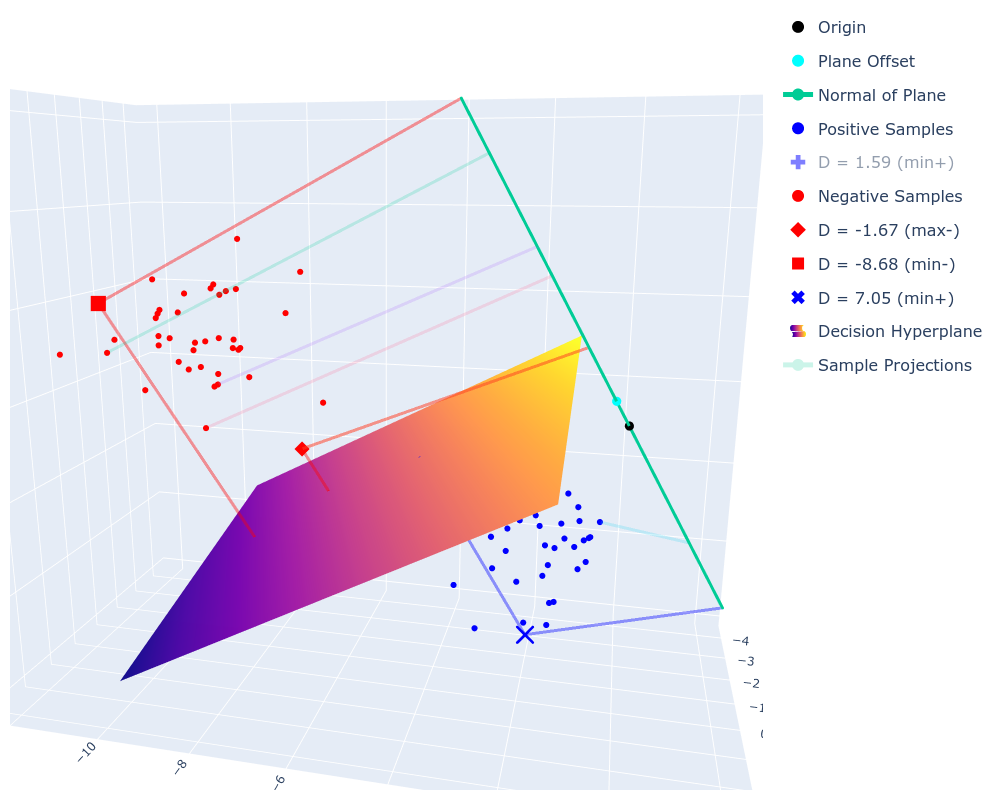
\includegraphics[width=0.9\textwidth]{3dplot_hyperplane_and_orthogonal}
	  \caption[Visual representation of the Hyperplane of an SVM splitting a dataset]{ \label{fig:3d_hyperplane_ortho} Visual representation of the Hyperplane of a Support-Vector-Machine splitting a dataset, as well as it's orthogonal and the orthogonal projection of a set of samples onto the plane. For an interactive version of this plot, visit  {\small \url{https://nbviewer.org/github/cstenkamp/derive_conceptualspaces/blob/main/notebooks/text_referenced_plots/hyperplane_orthogonal_3d.ipynb?flush_cache}}}
	\end{center}
\end{figure}


\includeMD{pandoc_generated_latex/section_algorithm}


\subsection{Preprocessing}

There are issues with using stop-word lists, see \cite{nothman-etal-2018-stop} ( SkLearn references this paper why their own/stopwordslists in general suck)


%Was für Schritte hat der Algo 

%TODO something along the lines of "Da, based on [source die die accuracy von dem gtranslate algorithm mit denen von menschen vergleicht], a gtranslate translation is as good as the average lecturer, it is assumed that translating the texts to english before using an english model can lead to better results


\subsection{Extracting Candidate Terms}
\label{sec:extract_candidates}

* KeyBERT

%TODO theoretisch ist es auch möglich bspw nen network mit attention auf gewisse dinge wie fachbereich und anderes zu trainieren und dann rauszusuchen was die wichtigen ausschlaggebenden dinge für das Netzwerk waren

%TODO extract using TF/IDF as well

%TODO a source: https://github.com/MaartenGr/KeyBERT#citation

* After you figure out which candidate term appears in which texts, figure out which other terms are frequent in these texts while infrequent in texts of the other class and then add these to the candidate-term-set (other way may even be to classify the texts according to if the candidateterm appears in them, and then take the misclassified one also as positive samples)

\begin{figure}[H]
	\centering
	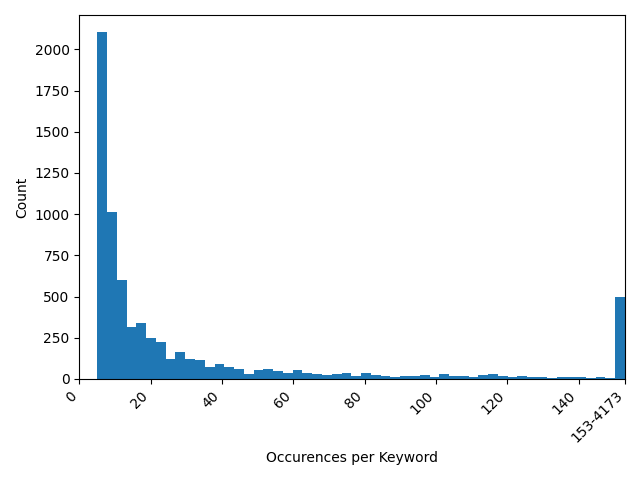
\includegraphics[width=\figwidth]{graphics/figures/keyphrases_histogram.png}
	%plot created with scripts/create_siddata_dataset.py filter-keyphrases /home/chris/Documents/UNI_neu/Masterarbeit/DATA_CLONE --verbose
	\caption[Occurences in all Documents per Keyphrase]{
		\label{fig:keyphrases_histogram}
		Occurences in all Documents per Keyphrase (for all keyphrases that occur $\geq$ 5 times, cut off at the 93th percentile).
		7007 of 45295 terms occur at least 5 times.
		Most frequent phrases: seminar (4173), course (3722), students (2923), it (2671), language (2071), work (1980), event (1842), research (1731), lecture (1723), law (1719).
		}
\end{figure}


\subsection{Calculating the distance to the SVMs Separatrix}
\label{sec:calculate_distance}

%TODO: before this, explain 
% * extraction of the candidate term set
% * how vectors are made from texts
In order to tell how much a text is prototypical of a category, all texts are split depending on whether they contain words of a set as described in \ref{sec:extract_candidates}, before a linear Support Vector Machine Classifier is trained on the vector-representation of all of the texts, splitting them into two classes: those that contain one of the candidate terms and those that do not. Due to the linear kernel, the SVM finds a hyperplane (\textit{separatrix}) that splits the positive from the negative samples in a way that maximizes the distance between the respective classmembers and the separatrix, using samples close to the margin as \textit{support vectors}. %TODO: what if the data is not linearly seperable?

Following the SVMs logic, one could argue that the further away a sample is from this separatrix, the more prototypical it is of its class. Thus, the distance of a sample to its \textit{orthogonal projection onto the hyperplane} %TODO explain orthogonal projection
may serve as metric for how prototypical a sample is for the respective category. 

Translated into terms relevant to the aim of this thesis, the classes may be those educational resources whose description contains the word "\textit{hard}" as one class vs. those that do not as the other class. Now according to [TODO], one may use the distance of the sample towards the separatrix as a measure of how hard a class is: For all positive samples, a longer distance means a harder class, for all negative samples a longer distance means an easier one, whereas those samples close to the separatrix can be considered average.

\subsubsection*{How to calculate the distance}

%TODO mention that I'm in a cartesian coordinate system
%TODO mention that I'm thinking in euclidian coordinates, see https://en.wikipedia.org/wiki/Plane_(geometry)
\noindent In the following paragraphs, I will visualize how to calculate the orthogonal distance from a sample to the hyperplane exemplary for the case of three-dimensional text-vectors.

Generally, the separatrix splitting positive from negative samples for an $n$-dimensional space $\mathds{R}^n$ is an $n-1$-dimensional subspace (called \textit{hyperplane}), which in the case of $\mathds{R}^3$ corresponds to a plane. 
%https://en.wikipedia.org/wiki/Plane_(geometry)#Representation

The general form of the equation of a plane is given as the following linear equation, where parameters $a, b, c$ and $d$ encode the position of the plane:

\begin{equation}
	\label{eq:general_plane}
	ax + by + cz = d
	%TODO source? mein Tafelwerk? :D
\end{equation}

This reads as "All points $(x,y,z)$ for which \ref{eq:general_plane} holds are on the plane". 

In this representation of the plane, the vector $(a,b,c)$ encodes a normal vector orthogonal to this plane, whereas $d$ serves as intercept, encoding the intersection of plane and normal. (specifically: the perpendicular distance you would need to translate the plane along its normal to have the plane pass through the origin) In higher dimensions, the formula for the hyperplane would become $a_1x_1+a_2x_2+a_3x_3+...+a_nx_n = b$, which means that encoding the hyperplane for a space $\mathds{R}^n$ requires $n+1$ parameters.
% one rough quote in this paragraph from https://stackoverflow.com/a/17661431

%TODO explain that it's not even harder in higher-dimensional spaces
%TODO explain that nicely, in python the separatrix is perfectly specified using the normal and the intercept, so we have everything we need 
%TODO die handschriftlichen notizen aus den beiden notebooks einbauen
%TODO die plots aus dem notebook einbauen

% The distance from any point of this $\mathds{R}^n$ to the hyperplane is then calculated as the length of the vector that is the \textit{orthogonal projection} from that point onto the hyperplane. The orthogonal projection from one vector onto another can be calculated as 

% \begin{equation}
% 	\label{eq:orthogonal_projection}
% 	\hat{\vec{a}} = \frac{\vec{a}\cdot\vec{b}}{\vec{b}\cdot\vec{b}}\cdot\vec{b}
% 	%TODO source https://en.wikipedia.org/wiki/Vector_projection
% \end{equation}

% ...as we however have a plane we want to project to, not a vector, what I wrote here is rather useless, isn't it?


The distance from any point of this $\mathds{R}^n$ to the hyperplane can then be calculated as 
% As... * dist(point, point_projected_onplane)     						 (`project[1,3]_pre`)
%       * abs(trafo(point)[0])     										 (`protoypicality_pre`)
%       * np.dot(plane.normal, point) + plane.d							 (`project2_pre')
% ...normiert sind die alle gleich, aber for some reason differn die um nen multiplicator..?!
% And the projections...:
%       * back_trafo([0, trafo(point)[1], trafo(point)[2]]
% 		* plane.project(point): k = (ax+by+cz+d)/(a²+b²+c²); result = [x-ka, y-kb, z-kc]
%       * point - distance * plane.normal  (...aber nur mit protoypicality_pre als distance! )
% 		...note that second and third are basically equal - both calculate "how much do I need to go into the direction of the orthogonal" and then do so  (point - distance * normal). The difference is that in plane.project the distance is divided by (a²+b²+c²). Originally sagt der typ von SO (https://stackoverflow.com/a/17661431) die distance ist einfach n*p-d, dann fehlt nur der normierungsterm. 
% TODO: figure out the explanation of the difference from this to the result of using forward and backward??
% See get_svm_decisionboundary.ipynb, den kram zwischen `#deleteme from here', commit d46a8300dae81adee


\subsection{Clustering the extracted candidates}

An analysis of \cite{Carmel2009} showed that a statistical method to extract features from clustered text corpora identified the labels of human annotators as one of the top five most important terms in only 15\% of cases, implying ``that human labels are not necessarily significant from a statistical perspective" \cite[139]{Carmel2009}
%TODO: die eigentliche Methode (JSD) mehr erklären!!
%(the JSD method for feature selection identifies human labels as “significant” (appearing in the top five most important terms) for only 15% of the categories. This result implies that human labels are not necessarily significant from a statistical perspective.z)
